\documentclass[review]{elsarticle}

\usepackage{lineno,hyperref}
\modulolinenumbers[5]

\journal{Journal of \LaTeX\ Templates}

%%%%%%%%%%%%%%%%%%%%%%%
%% Elsevier bibliography styles
%%%%%%%%%%%%%%%%%%%%%%%
%% To change the style, put a % in front of the second line of the current style and
%% remove the % from the second line of the style you would like to use.
%%%%%%%%%%%%%%%%%%%%%%%

%% Numbered
%\bibliographystyle{model1-num-names}

%% Numbered without titles
%\bibliographystyle{model1a-num-names}

%% Harvard
%\bibliographystyle{model2-names.bst}\biboptions{authoryear}

%% Vancouver numbered
%\usepackage{numcompress}\bibliographystyle{model3-num-names}

%% Vancouver name/year
%\usepackage{numcompress}\bibliographystyle{model4-names}\biboptions{authoryear}

%% APA style
%\bibliographystyle{model5-names}\biboptions{authoryear}

%% AMA style
%\usepackage{numcompress}\bibliographystyle{model6-num-names}
\usepackage{amsmath}
\usepackage{psfrag}
\usepackage{graphicx}
\usepackage{epsfig}
\usepackage{epstopdf}


%% `Elsevier LaTeX' style
\bibliographystyle{elsarticle-num}
%%%%%%%%%%%%%%%%%%%%%%%

\newcommand{\paral}{\; \vert \;}
\newcommand{\myvec}[1]{\overrightarrow{#1}}
\newcommand{\Defeq}{\stackrel{\mathrm{df}}{=}}
\newcommand{\Bnfeq}{::=}
\newcommand{\Co}[1]{\overline{#1}}

%
\newcommand{\Bsep}{\: \mid \: }
\newcommand{\Rule}[2]{\displaystyle{\frac{#1}{#2}}}
\newcommand{\SF}[1]{\mathsf{#1}}
\newcommand{\Act}{\mathsf{Act}}
\newcommand{\Vis}{\mathsf{Vis}}
\newcommand{\ActK}{\mathsf{ActK}}
\newcommand{\Proc}{\mathsf{Proc}}
\newcommand{\Procc}{\mathsf{ProcC}}
\newcommand{\Pred}{\mathsf{Pred}}
\newcommand{\Std}{\mathsf{Std}}
\newcommand{\rms}{\mathrm{S}}
\newcommand{\rmrec}{\mathrm{rec}}
\newcommand{\rmreck}{\mathrm{reck}}
\newcommand{\rmreckR}{\mathrm{reckR}}
\newcommand{\rma}{\mathrm{A}}
\newcommand{\rmp}{\mathrm{P}}
\newcommand{\rmf}{\mathrm{F}}
\newcommand{\rmr}{\mathrm{R}}
\newcommand{\rmfr}{\mathrm{FR}}
\newcommand{\equivS}{\equiv_{\mathrm{S}}}
\newcommand{\SigSA}{\Sigma_{\mathrm{SA}}}
\newcommand{\ltran}[1]{\stackrel{#1}{\longrightarrow}}
\newcommand{\tran}[1]{\stackrel{#1}{\rightarrow}}
\newcommand{\nottran}[1]{\stackrel{#1}{\not\rightarrow}}
\newcommand{\Rtran}[1]{\stackrel{#1}{\rightsquigarrow}}
\newcommand{\notRtran}[1]{\stackrel{#1}{\not\rightsquigarrow}}
\newcommand{\trans}[1]{\stackrel{#1}{\rightarrow}_{\mathrm{S}}}
\newcommand{\Par}{\mid}
\newcommand{\restrict}[1]{\!\setminus\!#1}

\newcommand{\mA}{\mathcal{A}}
\newcommand{\mSA}{\mathcal{SA}}
\newcommand{\mWA}{\mathcal{WA}}
\newcommand{\mAK}{\mathcal{AK}}
\newcommand{\umAK}{\underline{\mathcal{A}}\mathcal{K}}
\newcommand{\un}[1]{\underline {#1}}
\newcommand{\PI}{\mathcal{PI}}
\newcommand{\rom}[1]{\mbox{\rm{#1}}}

\newcommand{\Nil}{\mathbf{0}}
\newcommand{\New}[1]{\nu#1\: }
\newcommand{\Str}{\equiv}
\newcommand{\stdpred}{\mathsf{std}}
\newcommand{\std}[1]{\mathsf{std}(#1)}
%
\newcommand{\Bch}[2]{\mathsf{before}_{#1}(#2)}

\newcommand{\keys}[1]{\mathsf{keys}(#1)}
\newcommand{\kkey}[1]{\mathsf{k}(#1)}
\newcommand{\key}[1]{[#1]}
\newcommand{\Keys}{\mathcal{K}}
\newcommand{\freshpred}[1]{\mathsf{fsh}[#1]}
\newcommand{\fresh}[2]{\mathsf{fsh}[#1](#2)}

\newcommand{\ta}[1]{\mathsf{ta}(#1)}
\newcommand{\action}[1]{\mathsf{act}(#1)}

\newcommand{\intr}{\mbox{\ $\hat{}$\ }}
%\newcommand{\intr}{\mbox{\; $\widehat{}$\;}}
\newcommand{\sterm}{\mathsf{trm}}
\newcommand{\Sterm}[1]{\sterm(#1)}
\newcommand{\und}[1]{\underline{#1}}
\newcommand{\sqc}{\mathop{\cdot}}
\newcommand{\card}[1]{|#1|}
\newcommand{\bydef}{\stackrel{\emph{def}}{=}}
%
\newcommand{\Angle}[1]{\langle #1 \rangle}
\newcommand{\Tri}{\triangleright}
\newcommand{\Hole}{\bullet}
\newcommand{\rec}[1]{\mathrm{rec}\, #1}
\newcommand{\Rec}[1]{\rec #1 .}
\newcommand{\Rch}{\mathsf{Rch}}
\newcommand{\prune}{\pi}
\newcommand{\Prune}[1]{\prune(#1)}
\newcommand{\Root}[1]{\mathsf{rt}(#1)}

\newcommand{\Bis}{\sim}
\newcommand{\Biss}{\Bis_{\mathsf{S}}}
\newcommand{\Bisf}{\Bis_{\mathsf{F}}}
\newcommand{\Bisfr}{\Bis_{\mathsf{FR}}}
%\newcommand{\Bisu}{\Bis_{\Un}}
\newcommand{\Sim}{\mathcal{S}}
\newcommand{\Rem}{\backslash}
\newcommand{\sqeqt}{\sim}
% rules:
% static rule
\newcommand{\one}{\mbox{(I)}}
\newcommand{\onef}{\mbox{(1)}}
\newcommand{\oner}{\mbox{(1R)}}
% choice rule
\newcommand{\two}{\mbox{(II)}}
\newcommand{\twof}{\mbox{(2)}}
\newcommand{\twor}{\mbox{(2R)}}
% choice axiom
\newcommand{\thr}{\mbox{(III)}}
\newcommand{\thrf}{\mbox{(3)}}
\newcommand{\thrr}{\mbox{(3R)}}
\newcommand{\thrpf}{\mbox{(3\,$'$\!)}}
\newcommand{\thrpr}{\mbox{(3\,$'$\!R)}}
%
%
\newcommand{\Draft}[1]{}
\newcommand{\Comment}[1]{}
\newcommand{\Rev}[1]{{#1}^{-1}}
\newcommand{\rulename}[1]{\textsf{#1}}

\newtheorem{theorem}{Theorem}
\newtheorem{definition}{Definition}
\newtheorem{remark}{Remark}
\newtheorem{example}{Example}
\newtheorem{proposition}{Proposition}


\begin{document}

\begin{frontmatter}

\title{Elsevier \LaTeX\ template\tnoteref{mytitlenote}}
\tnotetext[mytitlenote]{Fully documented templates are available in the elsarticle package on \href{http://www.ctan.org/tex-archive/macros/latex/contrib/elsarticle}{CTAN}.}

%% Group authors per affiliation:
\author{Elsevier\fnref{myfootnote}}
\address{Radarweg 29, Amsterdam}
\fntext[myfootnote]{Since 1880.}

%% or include affiliations in footnotes:
\author[mymainaddress,mysecondaryaddress]{Elsevier Inc}
\ead[url]{www.elsevier.com}

\author[mysecondaryaddress]{Global Customer Service\corref{mycorrespondingauthor}}
\cortext[mycorrespondingauthor]{Corresponding author}
\ead{support@elsevier.com}

\address[mymainaddress]{1600 John F Kennedy Boulevard, Philadelphia}
\address[mysecondaryaddress]{360 Park Avenue South, New York}

\begin{abstract}
This template helps you to create a properly formatted \LaTeX\ manuscript.
\end{abstract}

\begin{keyword}
\texttt{elsarticle.cls}\sep \LaTeX\sep Elsevier \sep template
\MSC[2010] 00-01\sep  99-00
\end{keyword}

\end{frontmatter}

\linenumbers

\section{Introduction}
Probably write this last, once we have the rest

\section{A Calculus of Covalent Bonding}\label{sec:calculus}

This is from socp paper, needs reworking

We define the set of (forward) action labels $\mA$ which is  
ranged over by $a,b,c,d,e$. We partition $\mA$ into the set of \emph{strong actions}, written as
$\mSA$, and the set of \emph{weak actions} $\mWA$. Reverse action labels belong to 
$\underline\mA$, with typical members $\un{a},\un b, \un c,\un d, \un e $, and represent 
undoing of actions. The set $\mathcal{P}(\mA \cup \underline\mA)$ is ranged over by $L$.

Let $\Keys$ be an infinite set of {\em communication keys} (or {\em keys}
for short), ranged over by $k,l, m,n$. The Cartesian product $\mathcal A \times \Keys$, denoted by $\mAK$,
represents past actions, which are written as $a[k]$ for $a\in \mA$ and $k\in\Keys$. 
Correspondingly, we have the set $\umAK$ that represents undoing of past actions. 
We use $\alpha, \beta$ to identify actions which are either from $\mA$ or $\mAK$. It will be 
useful to consider sequences of actions or past actions, namely the elements of $(\mA \cup \mAK)^*$, 
which are ranged over by $s,s'$ and sequences of purely past actions, namely the elements of $\mAK^*$, 
which are ranged over by $t,t'$. The empty sequence is denoted by $\epsilon$ and $\alpha:s$
is the sequence with the head $\alpha$ and the tail $s$.

We shall also use two sets of auxiliary action labels, namely the set $(\mA) =\{ (a)\ \mid a\in\mA\}$, 
and its product with the set of keys, namely $(\mA)\Keys$.

We now define a Calculus of Covalent Bonding, or CCB for sort. The syntax is given below, where 
$f:\mA \rightarrow \mA$. 
We have a set of process identifiers (constants) $\PI$, with typical elements $S,T$, which 
contains the deadlocked process $\Nil$. 
The set of CCB closed terms is denoted by $\Proc$. We shall refer to closed terms as processes, and  
let $P,Q, R$ to range over processes.
Each process identifier $S$ has a defining equation $S\bydef P$. 
$$\begin{array}{lll}
	P & ::= &  S \ \mid \ (s;b).P \ \mid \ P\paral Q \ \mid \ P\restrict L \ \mid \ P[f]
\end{array}$$
We have a prefixing operator
$(s;b).P$, where $s$ is a non-empty sequence of actions or past actions. 
The actions in $s$, which have not happened yet,
can happen in any order. The action $b$ is a weak action in $\mWA$ and it can only happen after all
actions in $s$ have taken place. 
Performing $b$ then forces undoing one of the past actions in $s$ 
(using the concert rule in Figure~\ref{fig:csos}).
The action after the $;$ in $(s;b).P$ can be omitted, in which case the prefixing 
is simply $(s).P$, and is the prefixing in \cite{PUY12}. In this form, one of the actions 
in $s$ may be a weak action from $\mWA$. If $s$ is
a single element sequence, then the action is a strong action in $\mSA$ and
the prefixing operator is the prefixing of CCS \cite{Mil80}. 
We often omit trailing $\Nil$s so, for example, $(s).\Nil$ is written as $(s)$. All actions in 
$s$ in $(s;b).P$ are strong actions (in $\mSA$).

$P\paral Q$ represents processes $P$ and $Q$ which can perform actions or reverse actions on
their own, or which can interact with each other according to a communication function
$\gamma$ (much like in ACP \cite{BW90}). Or, they can perform a pair of the so-called \emph{concerted actions},
which is the new feature of our calculus.
We also have the usual restriction (encapsulation) operator
$\setminus L$, where $L$ is a set of labels, and the relabelling operator $[f]$.

The forward and reverse SOS rules for CCB are in 
Figures~\ref{fig:fsos}-\ref{fig:sc}, where
the rules in Figures~\ref{fig:fsos}-\ref{fig:reversesos}
are influenced by \cite{PhiUli07}. Since we do not use the relabelling operator in the systems modelled in 
this paper, we omit all SOS rules for $[f]$.
Note that the reverse rules in Figure~\ref{fig:reversesos}
are simply the symmetric versions of the corresponding forward rules. 

We use two predicates, $\std{P}:\mathcal{P}(\Proc)$ and $\fresh{m}{P}:\mathcal{P}(\Keys \times 
\Proc)$ in our SOS rules. They are defined in Figure~\ref{fig:predicates}. Two further auxiliary 
functions, 
$\kkey{i}: (\mathcal{A}\cup\mathcal{AK})^* \rightarrow \mathcal{P}(\Keys)$ and $\keys{P}: \Proc 
\rightarrow \mathcal{P}(\Keys)$, are also used. The function $\kkey{}$ is defined as follows:
$ \kkey{\epsilon}=\emptyset$;  $\kkey{\alpha:s}= \{l\}\cup\kkey{s}$ if $\alpha=a[l],a\in \mathcal{A},l \in \Keys$;
and $\kkey{\alpha:s}= \kkey{s}$ if $\alpha \in \mathcal{A}$.
The function $\keys{}$ is defined as $\keys{\Nil}=\emptyset$; $\keys{S}=\keys{P}$ if $S\bydef P$;
$\keys{(s;b).P}=\kkey{s} \cup \kkey{b} \cup \keys{P}$; 
$\keys{P \paral Q}= \keys{P} \cup \keys{Q}$; and $ \keys{P \restrict L}=\keys{P}$.
Informally $\keys{P}$ associates with each $P$ the set of its keys. A process $P$ is standard, 
written $\std{P}$, if it contains no past actions. A key $n$ is fresh in $Q$, written $\freshpred{n}(Q)$, 
if $n$ is not used in $Q$. We extend the notion of fresh keys to the sequences of actions and 
past actions $s$ and $t$ via the function $\kkey{}$.


The semantics of CCB is given by the labelled transition system (lts),
$$ (\Proc, L,\rightarrow: \subseteq \Proc \times L \times \Proc)$$
where the set of action labels $L$ is $\mAK \cup \umAK \cup (\mAK \times \umAK)$: it contains
the pairs of concerted actions $\mAK \times \umAK$ (see Figure~\ref{fig:csos}) as well as actions and past actions. 
The transition relation $\rightarrow$
is the least relation defined by our SOS rules and reduction rules in Definition~\ref{def:reduction}.

\renewcommand{\arraystretch}{3}
\begin{figure}[t]
\[
\begin{array}{l}
\Rule
{}
{\std{\Nil}}
\qquad; 
\Rule
{\std{P}}
{\std{S}}
\;\;
S \bydef P
\qquad 
\Rule   
{\kkey{s}=\emptyset \quad  \std{P}}
{\std{(s;b).P}}
\qquad 
\Rule   
{\std{P} \quad \std{Q}}
{\std{P \paral Q}}
\qquad
\Rule   
{\std{P}}
{\std{P \setminus L}}
\\%[12pt]
\Rule
{}
{\fresh{m}{\Nil}}
\quad \;
\Rule
{\fresh{m}{P}}
{\fresh{m}{S}}
\;\;
S \bydef P
\quad\; 
\Rule
{m \notin \kkey{s} \; m \neq n \; \fresh{m}{P}}
{\fresh{m}{(s;b[n]).P}}
\quad \;
\Rule
{m \notin \kkey{s} \quad \fresh{m}{P}}
{\fresh{m}{(s;b).P}}
\\%[12pt]
\Rule
{\fresh{m}{P} \quad \fresh{m}{Q}}
{\fresh{m}{P \paral Q}}
\qquad
\Rule
{\fresh{m}{P}}
{\fresh{m}{P \setminus L}}
\end{array}
\]
\caption{Predicates $\mathsf{std}$ and $\mathsf{fsh}$} \label{fig:predicates}
\end{figure}

\begin{figure}[t] 
\[
\begin{array}{ll}
\rom{act1}\ 
\Rule
{\std{X} \quad \fresh{k}{s}}
{(s,a;b).X \xrightarrow{a[k]}(s,a[k];b).X}
\qquad &
\rom{act2}\
\Rule
{X \xrightarrow{a[k]} X' \quad \fresh{k}{t}}
{(t;b).X \xrightarrow{a[k]} (t;b).X'}
\\
\rom{par}\
\Rule
{X \xrightarrow{a[k]} X'\quad \fresh{k}{Y}}
{X \paral Y \xrightarrow{a[k]} X' \paral Y}
\qquad &
\rom{com}\
\Rule
{X \xrightarrow{a[k]} X' \quad Y \xrightarrow{b[k]} Y'}
{X \paral Y \xrightarrow{c[k]} X' \paral Y'}
\; \gamma(a,b)=c
%
\\
\rom{res}\
\Rule
{X \xrightarrow{a[k]} X'}
{X\backslash L \xrightarrow{a[k]} X'\backslash L}
\; a \notin L
\qquad &
\rom{con}\
\Rule
{X \xrightarrow{a[k]} X'}
{S \xrightarrow{a[k]} X'}
\; S \bydef X
\end{array}
\] 
\caption{Forward SOS rules} \label{fig:fsos}
\end{figure}

\begin{figure}[t]
\[
\begin{array}{ll}
\rom{rev act1}\
\Rule
{\std{X} \quad \fresh{k}{s}}
{(s,a[k];b).X \xrightarrow{\underline{a}[k]}(s,a;b).X}
\quad &
\rom{rev act2}\
\Rule
{X \xrightarrow{\underline{a}[k]} X' \quad \fresh{k}{t}}
{(t;b).X \xrightarrow{\underline{a}[k]} (t;b).X'}
\\
\rom{rev par}\
\Rule
{X \xrightarrow{\underline{a}[k]} X'\quad \fresh{k}{Y}}
{X \paral Y \xrightarrow{\underline{a}[k]} X' \paral Y}
\qquad &
\rom{rev com}\
\Rule
{X \xrightarrow{\underline{a}[k]} X' \quad Y \xrightarrow{\underline{b}[k]} Y'}
{X \paral Y \xrightarrow{\underline{c}[k]} X' \paral Y'}
\; \gamma(a,b)=c
%
\\
\rom{rev res}\
\Rule
{X \xrightarrow{\underline{a}[k]} X'}
{X\backslash L \xrightarrow{\underline{a}[k]} X'\backslash L}
\; a \notin L
\qquad &
\rom{rev con}\
\Rule
{X \xrightarrow{\underline{a}[k]} X'}
{X \xrightarrow{\underline{a}[k]} S}
\; S \bydef X'
\end{array}
\]
\caption{Reverse SOS rules } \label{fig:reversesos}
\end{figure}

\begin{figure}[t] 
\[
\begin{array}{l}
\rom{aux1}\ 
\Rule{\std{X} \quad \fresh{k}{t}}
{(t;b).X \xrightarrow{(b)[k]}(t;b[k]).X}
\qquad\qquad
\rom{aux2}\
\Rule
{X \xrightarrow{(b)[k]} X' \quad \fresh{k}{t}}
{(t;a).X \xrightarrow{(b)[k]} (t;a).X'}
\\
\rom{concert}\ 
\Rule
{X\xrightarrow{(a)[k]}X' \quad X'\xrightarrow{\underline{b}[l]}X'' \qquad Y\xrightarrow{\alpha[k]}Y' 
  \quad Y'\xrightarrow{\underline{d}[l]}Y''% %\quad \fresh{k}{Y} 
 }
{X \paral Y\xrightarrow{\{e[k],\underline{f}[l]\}} X'' \paral Y''}\\%[8pt]
% \mbox{ if 1. } \alpha \mbox{ is } c \mbox{ or } (c) \mbox{ and } \gamma(a,c)=e \mbox{ for some } 
% c\in \mathcal{A} \mbox{, and 2. } \gamma(b,d)=f\\%[10pt]
\rom{concert act}\
\Rule
{X \xrightarrow{\{{a}[k], \underline{b}[l]\}} X' \quad \fresh{k}{t}}
{(t;a).X \xrightarrow{\{{a}[k], \underline{b}[l]\}} (t;a).X'}\\%[12pt]
\rom{concert par}\
\Rule
{X \xrightarrow{\{{a}[k], \underline{b}[l]\}} X'\quad \fresh{k}{Y}}
{X \paral Y \xrightarrow{\{{a}[k], \underline{b}[l]\}} X' \paral Y}\qquad
\rom{concert res}\
\Rule
{X \xrightarrow{\{{a}[k], \underline{b}[l]\}} X'}
{X\backslash L \xrightarrow{\{{a}[k], \underline{b}[l]\}} X'\backslash L}
%\;  a, b  \notin L \cup (L) 
% was \;  a, \underline{b}  \notin L \cup (L) 
%
\end{array}
\] 
\caption{SOS rules for concerted transitions. Rule concert applies if 1. $\alpha$ is $c$ or $(c)$
and $\gamma(a,c)=e$ for some $c\in \mathcal{A}$, and 2. $\gamma(b,d)=f$. Rule concert res applies
if $a, \underline{b}  \notin L \cup (L)$.}
\label{fig:csos}
\end{figure}

\begin{figure}[t] 
\[
\begin{array}{l}
\rom{sc}\
\Rule
{X \Rightarrow^* Y \quad Y \tran{\mu} Y' \quad Y' \Rightarrow^* X'}
{X\tran{\mu} X'} \qquad 
%
\rom{rev sc}\
\Rule
{X \Rightarrow^* Y \quad Y \tran{\underline{\mu}} Y' \quad Y' \Rightarrow^* X'}
{X\tran{\underline{\mu}} X'} \quad 
\end{array}
\] 
\caption{Structural congruence rules} \label{fig:sc}
\end{figure}
\renewcommand{\arraystretch}{1}

Figure \ref{fig:csos} contains the rule concert that defines when a pair of concerted actions 
takes place. We also have two auxiliary rules aux1 and aux2 which define the auxiliary 
transition relations needed in the concert rule. Note that aux1 and aux2 define transitions 
with the auxiliary labels $(b)[k]$ for all $(b) \in \mA$ and $k \in \Keys$.  Overall, 
transitions are labelled with $a[k] \in \mAK$, or with $\underline{b}[l] \in \umAK$, or with 
concerted pairs $\{a[k], \underline{b}[l]\}$.
Note that the concert rule uses \emph{lookahead} \cite{Uli92}.

We also need a reduction relation to define \emph{promotion} of actions. 
First we define {\em free names} of processes.

\begin{definition} \normalfont 
Function $\mathsf{fn}$, with $\mathsf{fn}: \Proc \rightarrow \mathcal{P}(\Keys)$, is defined as follows: $\mathsf{fn}(\Nil) = \emptyset$, $\mathsf{fn}(S)=\mathsf{fn}(P) \text{ if }  S\bydef P$, $\mathsf{fn}((\alpha : s;b).P)=\{\alpha\} \cup \mathsf{fn}(s;b).P)$, $\mathsf{fn}((a;b).P)=\{a,b\} \cup \mathsf{fn}(P) $, $\mathsf{fn}(P\paral Q)=\mathsf{fn}(P) \cup \mathsf{fn}(Q)$ and $\mathsf{fn}(P \restrict L)=\mathsf{fn}(P) \restrict L$.
\end{definition}

\begin{definition}\label{def:reduction}{\rm The reduction relation $\Rightarrow$ is the smallest 
reflexive and transitive binary relation that satisfies the following rules: 
$(\rom{red1})\; P\Par Q \Rightarrow Q\Par P$, (\rom{red2})\; $P\Par (Q\Par R) \Rightarrow 
(P\Par Q)\Par R$, (\rom{red3})\; $(P\Par Q)\Par R \Rightarrow P\Par (Q\Par R)$, (\rom{red4})\;
$P\Par \Nil \Rightarrow P$, (\rom{red5})\; $(P\paral Q)\backslash L \Rightarrow P\backslash L 
\paral Q$  if $\mathsf{fn}(Q) \cap L = \emptyset$, (\rom{red6})\; $P\backslash L \paral Q \Rightarrow 
(P\paral Q)\backslash L$  if $\mathsf{fn}(Q) \cap L = \emptyset$, (\rom{red7})\; $(s;b).P 
\backslash (s';b).P$ if $s'$ is a permutation of $s$, (\rom{prom})\; 
$(a:t;b[k]) \Rightarrow (a[k]:t;b)$ if $a \in \mathcal{SA}, b \in \mathcal{WA}$, 
(\rom{move})\; $(a:b[k]:s) \Rightarrow (a[k]:b:s)$ if  
$a \in \mathcal{SA}, b \in \mathcal{WA}$, where $t\in \mAK^*$ and $s\in (\mA \cup \mAK)^*$.
}
\end{definition}
%
We have two promotion rules in Definition~\ref{def:reduction}. The rule prom
promotes a weak bond to a strong bond. Since weak bonds are only temporary they get replaced by bonds 
on strong actions as soon as these become available. In more detail, after a bond is created on the
weak action $b$ another bond is broken at the same location involving a strong action, here $a$.  
This pair of concerted actions $\{b[k],a[l]\}$, for some $l$, results in $(a:t;b[k])$, which is
subjected immediately to bond promotion from a weak $b$ to a strong $a$, giving us $(a[k]:t;b)$.
Now weak $b$ can bond again. We have another rule move which promotes correspondingly 
a weak bond $b$ to a strong $a$.
In order to model what happens in chemical reactions more faithfully, we assume that prom and move
are used as soon as they become applicable.

This can be defined more formally by using the idea of Ordered SOS rules, suggested in \cite{irek2002} and \cite{mousavi}. For our purposes a partial ordering of SOS rules and structural congruence rules is appropriate. Figure~\ref{fig:osos} gives the partial ordering, where the rules in the upper field have precedence over the rules in the lower field. Note that we extend the original work by including congruence rules. We only have positive premises, which avoids problems of combining negative premises with ordering.

\begin{figure}
\[
\begin{array}{|c||c|}
\downarrow & \rom{red1}, \rom{red2}, \rom{red3}, \rom{red4}, \rom{red5}, \rom{red6}, \rom{red7}, \rom{prom}, \rom{mov}, \rom{sc}, \rom{rev sc} \\
\hline
& \rom{act1}, \rom{act2}, \rom{par}, \rom{com}, \rom{res}, \rom{con}, \rom{rev act1}, \rom{rev act2}, \rom{rev par}, \\
& \rom{rev com}, \rom{rev res}, \rom{rev con}, \rom{concert}, \rom{concert par}, \rom{concert act}, \rom{concert res} 
\end{array}
\] 
\caption{Structural congruence rules} \label{fig:osos}
\end{figure}

We also have the usual structural congruence rules 
(sc and rev sc) in Figure~\ref{fig:sc}, where $\mu \in \mAK\cup \umAK \cup (\mAK\times \umAK) $, 
which combine potentially several reductions (including prom reductions) with transitions.

\begin{definition} \normalfont A process $P$ is \emph{consistent} if $\std{P}$ or $Q \rightarrow^* P$ 
for some process $Q$ such that $\std{Q}$.
\end{definition}

\begin{example}\label{ex:examp1}
Consider the process $(a;b) \paral a \paral b$ with $\gamma(a,a)=c$ and $\gamma(b,b)=d$. After the
initial synchronisation of actions $a$, which produces the transition $c[1]$, we have a transition 
with a pair of concerted actions by rule concert in Figure~\ref{fig:csos}
$$(a[1];b) \paral a[1] \paral  b \xrightarrow{\{d[2], \underline{c}[1]\}} 
  (a;b[2])\paral a \paral b[2]$$
since $(a[1];b) \xrightarrow{(b[2])} (a[1];b[2])\xrightarrow{\underline{a}[1]} (a;b[2])$ 
and $a[1] \paral b \xrightarrow{b[2]} a[1] \paral b[2] \xrightarrow{\underline{a}[1]} a \paral b[2]$.
\end{example}

\begin{example}\label{ex:examp2}
Consider $(a[1];b)\paral (a[1];b)\paral e$ with $\gamma(a,a)=c$ and $\gamma(b,b)=d$. 
We clearly have the following pair of concerted actions
 $$(a[1];b)\paral (a[1];b)\paral e  \xrightarrow{\{d[2], \underline{c}[1]\}} 
(a;b[2])\paral (a;b[2])\paral e. $$
\end{example}

There are processes with weak actions that can potentially communicate but there are no concerted actions
due to our SOS rules:

\begin{example}\label{ex:examp3}
Consider $(a[1];b)\paral (e[2];b)\paral (a[1],e[2])$ with $\gamma(a,a)=c$ and $\gamma(b,b)=d$.
It cannot perform any concerted actions: Although $(a[1];b)  \xrightarrow{(b)[l]} 
\xrightarrow{\underline{a}[1]} (a;b[l])$, for any $l$ different from 1 and 2, but 
$(e[2];b)\paral (a[1],e[2])$  cannot perform the $(b[l])$
transition since there are no SOS rules for parallel composition and auxiliary actions $(b)$. This forces us
to treat $(a[1];b)$ and $ (e[2];b)$ as $X$ and $Y$ in the concert rule, respectively, and we notice that
we cannot undo a communication on $a$ or $e$.
\end{example}


\begin{example}\label{example4}
The transition 
$(a[1];b) \paral a[1] \paral  b \xrightarrow{\{d[2], \underline{c}[1]\}} (a;b[2])\paral a \paral b[2]$ 
from Example \ref{ex:examp1} is followed by the application of the reduction rule prom that moves the bond 2
from the weak $b$ to the strong $a$:
$$(a;b[2])\paral a \paral b[2] \Rightarrow (a[2];b)\paral a \paral b[2] $$
As a result, we can bond on the weak $b$ again and, importantly, the $a[2]$ to $b[2]$ bond is irreversible
as $\gamma(a,b)$ is undefined. Note that reaching
this bond by computing forwards alone is not possible.
\end{example}

\section{Base Excision Repair}
\label{sec:ber}

\subsection{Description of Base Excision Repair}

This is from my thesis

So far we have seen some applications of CCB, which are very close to the original inspiration of the calculus. If the principles behind CCB are of some general relevance, there should be other processes we can model using our calculus. A candidate for these might be biological processes. These are ultimately chemical reactions, but they are often viewed at a much higher level of abstraction then we have done so far. Typically, in such studies atoms would no longer play a r\^{o}le, but proteins and other macromolecules, consisting of thousands or more atoms are considered as entities. Typical examples are pathways, gene regulation, transcription, or DNA repair. One of the mechanisms for DNA repair is \emph{base excision repair} (BER). Specifically, BER is responsible for repairing small damages, where a single base pair in the DNA is not correct. Such damages can be inflicted by processes in the body or various external factors like radiation. Repair of such damages is important to prevent a degradation of the DNA information in the organism. There are various subtypes of BER, and various proteins involved in it. For our purposes, we look at the case that a uracil base has been incorporated in the DNA. Uracil is normally only found in RNA, whereas DNA consists of the four bases adenine (A), cytosine (C), guanine (G), and thymine (T).

Uracil-DNA glycosylase (UNG or UDG) is the protein responsible for removing uracil from DNA and making the position available for insertion of the correct base. The process has been extensively studied\footnote{A good overview is given in \cite{pmid25252105}. We use a highly simplified view here. For example, there is not a single UDG, but a family of UDGs all exhibiting slightly different behaviour.} and modelled in \cite{Koehler2014} and \cite{kappadna}. A description of the process on an abstract level is as follows: UDG can bind to any of the deoxyribose/phosphate groups forming the backbone strands of the DNA. From there it can ``walk'' along the chain to the next deoxyribose/phosphate group (that walk makes it much more likely to find a damage than if UDG would just randomly bind to and get off the DNA strand again). If the base attached to this group is uracil, UDG will bind to it and dissolve the bond from the uracil to the DNA. Uracil can then be released and UDG can either continue the search or get off the DNA strand. The correct base can take the place of the uracil.

\subsection{Modelling BER}

In order to model BER, we need the following components: deoxyribose/phosphate groups, the UDG, the uracil and the four other bases. The other bases will not take part in the reactions, but include them in our model in order to demonstrate the interaction we. The components are the following:
%
$$\begin{array}{lll}
DP & \bydef & (p3,p5,b,d).DP'\\
UDG & \bydef & (h;f).(e).UDG'\\
U & \bydef & (b;e).(u).U'\\
A & \bydef & (b;i).(a).A'\\
T & \bydef & (b;i).(t).T'\\
G & \bydef & (b;i).(g).G'\\
C & \bydef & (b;i).(c).C'\\
\end{array}$$
%
where processes $A$, $T$, $G$, $C$, and $U$ model the bases adenine (A), cytosine (C), guanine (G), thymine (T), and uracil (U) respectively. Process $UDG$ represents the Uracil-DNA glycosylase and $DP$ a deoxyribose/phosphate group. Here $d$, $e$, $i$, and $f$ are weak actions, all other actions, namely $p3$, $p5$, $h$, $b$, $u$, $a$, $t$, $g$, and $c$ are strong.

The synchronisation function for our system is as follows:
%
$$\begin{array}{ l c l l }
\gamma(p3,p5) & = & p & \\
\gamma(b,b) & = & bb &\\
\gamma(a,t) & = & at &  \\
\gamma(g,c) & = & gc & \\
\gamma(h,d) & = & hd & \\
\gamma(f,d) & = & fd & \\
\gamma(e,e) & = & ee & \\
\end{array}$$
%
\begin{figure}[h!]
\psfrag{UDG}{${\mathrm{UDG}}$}
\psfrag{sp1}{${\mathrm{DP_1}}$}
\psfrag{sp2}{${\mathrm{DP_2}}$}
\psfrag{sp3}{${\mathrm{DP_3}}$}
\psfrag{sp4}{${\mathrm{DP_4}}$}
\psfrag{sp5}{${\mathrm{DP_5}}$}
\psfrag{sp6}{${\mathrm{DP_6}}$}
\psfrag{A}{${\mathrm{A}}$}
\psfrag{T}{${\mathrm{T}}$}
\psfrag{C1}{${\mathrm{C_1}}$}
\psfrag{C2}{${\mathrm{C_2}}$}
\psfrag{G1}{${\mathrm{G_1}}$}
\psfrag{G2}{${\mathrm{G_2}}$}
\psfrag{U}{${\mathrm{U}}$}
\psfrag{hd}{$hd$}
\psfrag{fd}{$fd$}
  \centering
    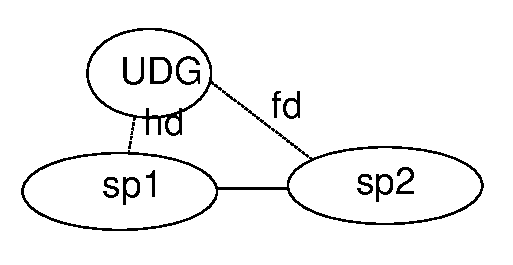
\includegraphics[width=1.0\textwidth]{ber/berintermediate}
  \caption[A $UDG$ unit whilst performing a step along a DNA strand.]{A $UDG$ unit whilst performing a step along a DNA strand. The $hd$ bond is broken together with the new $fd$ being formed.}
  \label{fig:berintermediate}
\end{figure}

We model the deoxyribose/phosphate groups first. This has two ends, normally called 3' and 5', which we model as $p3$ and $p5$ actions respectively. They help us to build the DNA strands. Also, there is a $b$ action, which enables binding of a base. Then we need a possibility for the UDG to bind and to ``walk'': this is enabled by actions $d$, $h$, and $f$, as we will see. UDG is modelled to have the prefix $(h;f)$, which enables the walk, since the strong action $h$ can be bonded to a $DP$ and $f$ can interact with a neighbouring $DP$. This breaks the $hd$ bond, and the $fd$ bond is then promoted to $d$, which gives us the $UDG$ being bonded to the neighbouring $DP$ the same way it was bound before to the other $DP$. Figure~\ref{fig:berintermediate} shows this intermediate situation whilst this step is performed. The five bases ($C$, $G$, $T$, $A$) all have a $b$ action to bind to a $DP$. If $A-T$ respectively $C-G$ are opposite each other they can bind and therefore form a correct base pair in the DNA. Uracil ($U$) is not able to form a base pair in our DNA context. All bases have a weak action in the prefix $(b;x)$. This action $x$ serves for removing the base from the DNA by breaking the $b$ bond. For uracil the action $x$ is $e$, for other bases it is $i$. By this UDG can be specific to uracil. In our model no action interacts with $i$, but of course other proteins not modelled might react with it. Note that $i$ and $e$ actions in the $U$, $A$, $T$, $G$, and $C$ processes cannot happen if the $u, a, t, g$ respctively $c$ actions are done, so $i$ and $e$ are blocked by $u, a, t, g,$ and $c$. Since $u, a, t, g$ and $c$ are used to form the base pairs this means that a correct base pair cannot be removed from the DNA in any case. This models the situation we need for the repair mechanism to work. We have used concerted actions in two instances here: Firstly to enable the UDG walk. This is an instance where backtracking would not work, since we need out-of-causal-order reversibility in this case. We cannot unbond from the old DP first and then choose the next $DP$, but we must hold the old bond until the new bond is formed. Secondly, we use a concerted action to enable the repair mechanism by making a bonding on the repair action break the bond to DP.

In the synchronisation function, we have the interaction of $p3$ and $p5$ to form the strands, the $b$-$b$ interaction for binding the bases, the $h$-$d$ and $f$-$d$ interaction for the ``walk'', the $a$-$t$ and $g$-$c$ interactions for forming the base pairs, and the $e$-$e$ interaction for the repair action.

In order to model a strand of DNA, we restrict ourselves to three base pairs. This means we need six $DP$ processes and six bases. We put two ``correct'' base pairs and one containing a uracil base. An extra $C$ base must be available for replacing $U$. We also use subscripts to distinguish processes where there is more than one instance of the process. The system is modelled in CCB as follows:

$$\begin{array}{l}
(DP_1 \paral DP_2 \paral DP_3 \paral A \paral T \paral G_1 \paral G_2 \paral U \paral C_1 \paral C_2 \paral DP_4 \paral DP_5 \paral DP_6 \paral UDG) \\
\setminus\{p3, p5, d, b, a, t, g, e, u, c, h, f, i\} 
\end{array}$$ 

We leave out the restriction from now on for ease of reading. We number actions using subscripts where there is more than one instance, and set initial bonds as required. We get the following process:
%
\begin{flalign*}
&(p3_1,p5_1[1],d_1,b_1[5]).DP_1' \paral (p3_2[1],p5_2[3],d_2,b_2[4]).DP_2' \paral (p3_3[3],p5_3,d_3,b_3[9]).DP_3' \paral &&\\
&(b_1[5];i_1).(a[6]).A' \paral (b_2[7];i_2).(t[6]).T' \paral (b_3[8];i_3).(g_1).G_1' \paral  ((b_4[9];i_4).(g_2[10]).G_2'  \paral &&\\
&(b_5[4];e_2).(u).U' \paral (b_6[11];i_6).(c_1[10]).C' \paral (b_7;i_7).(c_2).C' \paral (p3_4,p5_4[12],d_4,b_4[7]).DP_4' \paral &&\\ &(p3_5[12],p5_5[13],d_5,b_5[8]).DP_5' \paral (p3_6[13],p5_6,d_6,b_6[11]).DP_6' \paral (h;f).(e_2).UDG'&&
\end{flalign*}
%
\begin{figure}[h!]
\psfrag{UDG}{${\mathrm{UDG}}$}
\psfrag{sp1}{${\mathrm{DP_1}}$}
\psfrag{sp2}{${\mathrm{DP_2}}$}
\psfrag{sp3}{${\mathrm{DP_3}}$}
\psfrag{sp4}{${\mathrm{DP_4}}$}
\psfrag{sp5}{${\mathrm{DP_5}}$}
\psfrag{sp6}{${\mathrm{DP_6}}$}
\psfrag{A}{${\mathrm{A}}$}
\psfrag{T}{${\mathrm{T}}$}
\psfrag{C1}{${\mathrm{C_1}}$}
\psfrag{C2}{${\mathrm{C_2}}$}
\psfrag{G1}{${\mathrm{G_1}}$}
\psfrag{G2}{${\mathrm{G_2}}$}
\psfrag{U}{${\mathrm{U}}$}
\psfrag{1}{${\mathrm{1}}$}
\psfrag{2}{${\mathrm{2}}$}
  \centering
    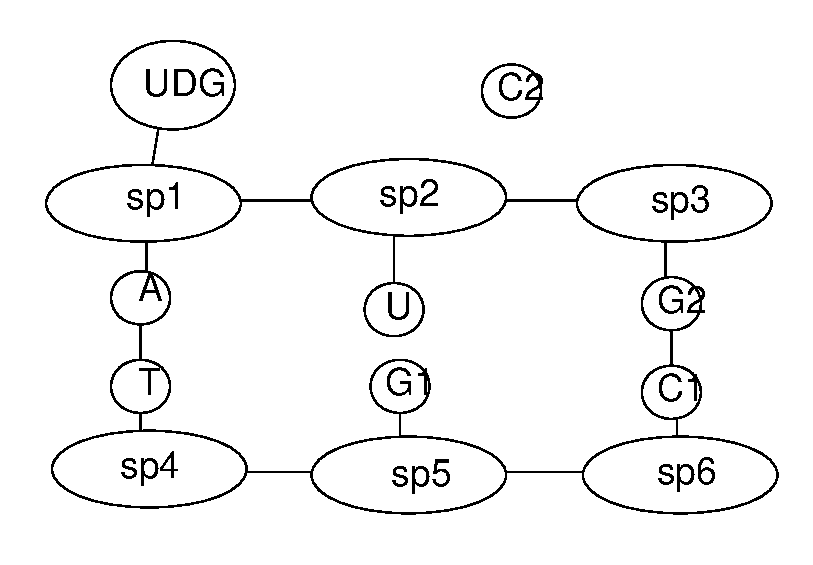
\includegraphics[width=1.0\textwidth]{ber/ber}
  \caption[A three base pair DNA fragment.]{A three base pair DNA fragment, with a uracil instead of a cytosine, and a UDG protein attached.}
  \label{fig:ber}
\end{figure}

Initially $UDG$ bonds to $DP_1$, which in turn is bonded to a correct base pair (note $UDG$ was not bound so far to any other process). The situation is shown in Figure~\ref{fig:ber} and is as follows (the bonds created, news keys and action on which keys were removed are shown in \textbf{bold}):
%
\begin{flalign*}
&\xrightarrow{hd[2]}(p3_1,p5_1[1],d_1\boldsymbol{[2]},b_1[5]).DP_1' \paral (p3_2[1],p5_2[3],d_2,b_2[4]).DP_2' \paral &&\\
&(p3_3[3],p5_3,d_3,b_3[9]).DP_3' \paral
(b_1[5];i_1).(a[6]).A' \paral (b_2[7];i_2).(t[6]).T' \paral (b_3[8];i_3).(g_1).G_1' \paral &&\\
&((b_4[9];i_4).(g_2[10]).G_2'  \paral (b_5[4];e_2).(u).U' \paral (b_6[11];i_6).(c_1[10]).C' \paral (b_7;i_7).(c_2).C' \paral &&\\
&(p3_4,p5_4[12],d_4,b_4[7]).DP_4' \paral (p3_5[12],p5_5[13],d_5,b_5[8]).DP_5' \paral &&\\
&(p3_6[13],p5_6,d_6,b_6[11]).DP_6' \paral (h\boldsymbol{[2]};f).(e_2).UDG'&&
\end{flalign*}
%
The UDG can now randomly ``walk'' along the chain. The $(h;f)$ prefix can appropriately model this, since if the weak $f$ action binds to the neighbour, the bond on $h$ is broken. In our case, action $f$ in $UDG$ can communicate with $d_2$ in $DP_2$. This breaks bond 2 from $h$ in $UDG$ to $d_1$ in $DP_1$, thus having performed a ``step''. We then move key $14$ from $f$ to $h$ (via the \rulename{prom} rule from Figure~\ref{fig:reduction}) and get:
%
\begin{flalign*}
&\xrightarrow{\{fd[14],\underline{hd}[2]\}} \Rightarrow (p3_1,p5_1[1],\boldsymbol{d_1},b_1[5]).DP_1' \paral (p3_2[1],p5_2[3],\boldsymbol{d_2[14]},b_2[4]).DP_2' \paral&&\\
&(p3_3[3],p5_3,d_3,b_3[9]).DP_3' \paral (b_1[5];i_1).(a[6]).A' \paral (b_2[7];i_2).(t[6]).T' \paral (b_3[8];i_3).(g_1).G_1' \paral&&\\
&((b_4[9];i_4).(g_2[10]).G_2'  \paral (b_5[4];e_2).(u).U' \paral (b_6[11];i_6).(c_1[10]).C' \paral (b_7;i_7).(c_2).C' \paral&&\\
&(p3_4,p5_4[12],d_4,b_4[7]).DP_4' \paral (p3_5[12],p5_5[13],d_5,b_5[8]).DP_5' \paral\\ &(p3_6[13],p5_6,d_6,b_6[11]).DP_6' \paral \boldsymbol{(h[14];f)}.(e_2).UDG'&&
\end{flalign*}
%
$UDG$ could now simply continue its walk, or it can interact via its $e$ action with the uracil. Note that other bases expose the $i$ action, so uracil cannot interact with them. The $u$, $a$, $t$, $g$, or $ c$ actions block $e$ or $i$, so correct base pairs are not affected by repairs. In our example $e_2$ on $UDG$ interacts with $e_2$ on $U$, breaking bond 4 between $b_5$ in $UDG$ and $b_2$ in $DP_2$. We have achieved the desired repair, since the uracil is removed from the DNA. We model this by the following transition (we use the rewrite rule again):
%
\begin{flalign*}
&\xrightarrow{\{ee[15],\underline{bb}[4]\}} \Rightarrow (p3_1,p5_1[1],d_1,b_1[5]).DP_1' \paral (p3_2[1],p5_2[3],d_2[14],\boldsymbol{b_2}).DP_2' \paral&&\\
&(p3_3[3],p5_3,d_3,b_3[9]).DP_3' \paral (b_1[5];i_1).(a[6]).A' \paral (b_2[7];i_2).(t[6]).T' \paral (b_3[8];i_3).(g_1).G_1' \paral&&\\
&((b_4[9];i_4).(g_2[10]).G_2'  \paral \boldsymbol{(b_5[15];e_2)}.(u).U' \paral (b_6[11];i_6).(c_1[10]).C' \paral (b_7;i_7).(c_2).C' \paral&&\\
&(p3_4,p5_4[12],d_4,b_4[7]).DP_4' \paral (p3_5[12],p5_5[13],d_5,b_5[8]).DP_5' \paral\\ &(p3_6[13],p5_6,d_6,b_6[11]).DP_6' \paral (h[14];f).(\boldsymbol{e_2[15]}).UDG'&&
\end{flalign*}
%
The floating $C_2$ can now take the place of the $U$ by binding to $DP_2$ and $G_1$. This is represented by the following two transitions:
%
\begin{flalign*}
&\xrightarrow{bb[16]}\xrightarrow{gc[17]}(p3_1,p5_1[1],d_1,b_1[5]).DP_1' \paral (p3_2[1],p5_2[3],d_2[14],\boldsymbol{b_2[16]}).DP_2' \paral&&\\
&(p3_3[3],p5_3,d_3,b_3[9]).DP_3' \paral (b_1[5];i_1).(a[6]).A' \paral (b_2[7];i_2).(t[6]).T' \paral (b_3[8];i_3).(\boldsymbol{g_1[17]}).G_1' \paral&&\\
&((b_4[9];i_4).(g_2[10]).G_2'  \paral (b_5[15];e_2).(u).U' \paral (b_6[11];i_6).(c_1[10]).C' \paral (\boldsymbol{b_7[16]};i_7).(\boldsymbol{c_2[17]}).C' \paral&&\\
&(p3_4,p5_4[12],d_4,b_4[7]).DP_4' \paral (p3_5[12],p5_5[13],d_5,b_5[8]).DP_5' \paral\\ &(p3_6[13],p5_6,d_6,b_6[11]).DP_6' \paral (h[14];f).(e_2[15]).UDG'&&
\end{flalign*}
%
The resulting process is shown in Figure~\ref{fig:ber2}.

\begin{figure}[h!]
\psfrag{UDG}{${\mathrm{UDG}}$}
\psfrag{sp1}{${\mathrm{DP_1}}$}
\psfrag{sp2}{${\mathrm{DP_2}}$}
\psfrag{sp3}{${\mathrm{DP_3}}$}
\psfrag{sp4}{${\mathrm{DP_4}}$}
\psfrag{sp5}{${\mathrm{DP_5}}$}
\psfrag{sp6}{${\mathrm{DP_6}}$}
\psfrag{A}{${\mathrm{A}}$}
\psfrag{T}{${\mathrm{T}}$}
\psfrag{C1}{${\mathrm{C_1}}$}
\psfrag{C2}{${\mathrm{C_2}}$}
\psfrag{G1}{${\mathrm{G_1}}$}
\psfrag{G2}{${\mathrm{G_2}}$}
\psfrag{U}{${\mathrm{U}}$}
\psfrag{1}{${\mathrm{1}}$}
\psfrag{2}{${\mathrm{2}}$}
  \centering
    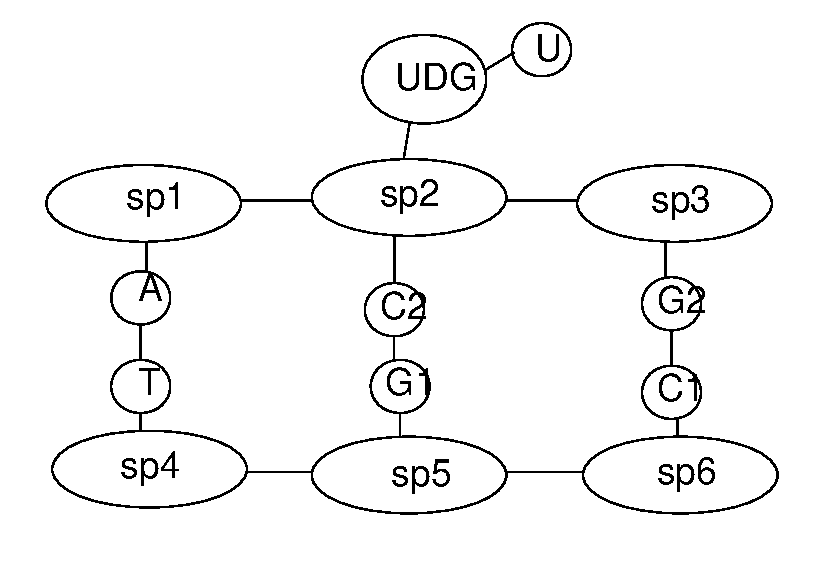
\includegraphics[width=1.0\textwidth]{ber/ber2}
  \caption[The repaired DNA fragment.]{The repaired DNA fragment, with the uracil replaced by a cytosine.}
  \label{fig:ber2}
\end{figure}

If uracil would have been bonded on $u$, the interaction with UDG could not have happened, so the defect is recognized. We now have the uracil broken from the deoxyribose/phosphate group and the $b$ action on the deoxyribose/phosphate group ready to bond to another base. UDG needs to release $U$ and then either to continue its walk or release itself from the DNA. We can again use our new operator for modelling UDG, since this way we achieve that the repair mechanism happens. On the other hand by combining two groups of actions we ``block'' this repair to happen if the desired second bond is there.

A limitation of our modelling is that it allows the UDG during its ``walk'' to bind to any DG group, since there is no restriction which $d$ action is used. In reality of course UDG must continue with the nearest DP group. This is a spatial effect our calculus does not model so far. Similarly, the repair by UDG binding to the $e$ action of a uracil (U) is not dependent on the UDG being next to it, whereas in reality it is. Again this is a spatial effect, which we will discuss in Section~\ref{sec:ccbs}.

We have used the software from Chapter~\ref{sec:simulation} to test the modelling. The desired path is one of the possibilities, which shows that our modelling is adequate in this respect. We also get some undesired reactions: Apart from UDG binding to any DP group during its walk, there is also the possibility that the unused $p5$ action of a $DP$, which is at the end of the DNA strand, interacts with an unused $p3$ from the a DP at the other end of the DNA strand. This is not impossible as a such, but prevented in reality by at least two effects we do not model. One is again the spatial arrangement, the other is the fact that the ends of the DNA are protected by special groups, which we do not model here. They prevent reactions at the DNA ends.

\subsection{Conclusion}

In this chapter we have seen that our calculus is suitable for modelling higher-level processes in biological systems. We have also used the full power of our calculus with nested prefixes like $(s;b).(s';b').P$, and not only simple processes of the form $(s;b).\Nil$, as we did before. We have modelled the ``walk'' of UDG along 
a strand of DNA by actions in $s$, and, once a fault is found, the repair mechanism was modelled
by the actions in $s'$. We have seen that our modelling enables some unwanted reactions, but we can explain this by noting that we do not include spatial effects in our modelling.

\section{Related Work}

\section{Future Work}

\section{Conclusion}

\section*{References}

\bibliography{mybibfile}

\end{document}